\documentclass[titlepage]{article}

\usepackage[utf8]{inputenc}
\usepackage[english]{babel} 
\usepackage{lineno, a4wide} % add line numbers
%\linenumbers
\usepackage{setspace} % to use double spacing
\doublespacing

\usepackage{authblk} % author and affiliations
\usepackage{amssymb, amsmath} % for math formulas
\usepackage{amsfonts} % blackboard math symbols
\usepackage[round]{natbib} % citation format
\usepackage{hyperref} % creates links in the document
\usepackage{doi} % Create correct hyperlinks for DOI numbers
\usepackage{times} %Select Adobe Times Roman (or equivalent) as default font

\usepackage{graphicx} % handling figures
\usepackage{subfig} % handling figures
\usepackage[nofiglist,figuresonly]{endfloat} % figures in the end
%\usepackage[nomarkers,figuresonly]{endfloat}
\usepackage{enumitem} % Control layout of itemize, enumerate, description
\usepackage{xcolor} % colored fonts

\usepackage[colorinlistoftodos]{todonotes} % to do comments

\usepackage{subfiles}
\usepackage{parskip}
\usepackage{multirow}
\usepackage[para,online,flushleft]{threeparttable}
\usepackage{rotating}
\usepackage{tikz}
\usepackage{tcolorbox}
\usepackage[export]{adjustbox}[2011/08/13]

\title{
Estimating cumulative effects and zones of influence from multiple anthropogenic infrastructure on biodiversity  \\
{\normalsize Submitted for review}
}

% authors
\author[1,2,*]{Bernardo Brandão Niebuhr}
\author[1,*]{Bram Van Moorter} 
\author[1]{Manuela Panzacchi}
\author[3]{Torkild Tveera}
\author[3]{Knut Langeland}
\author[4]{Audun Stien}
\author[1]{Olav Strand}
\author[5]{Per Sandström}
\author[2]{Anna Skarin}
\author[6]{Moudud Alam}

% affiliation
\affil[1]{Norwegian Institute for Nature Research (NINA), Trondheim, Norway}
\affil[2]{Swedish University of Agricultural Sciences (SLU), Uppsala, Sweden}
\affil[3]{Norwegian Institute for Nature Research (NINA), Tromsø, Norway}
\affil[4]{University of Tromsø, Tromsø, Norway}
\affil[5]{Swedish University of Agricultural Sciences (SLU), Umeå, Sweden}
\affil[6]{Dalarna University, Falun, Sweden}
\affil[*]{Joint first authorship}

\date{Corresponding author: Bernardo Brandão Niebuhr \\Norwegian Institute for Nature Research, Postboks 5685 Torgarden, \\7485 Trondheim, Norway \\Contact: bernardo.brandao@nina.no, bernardo\_brandaum@yahoo.com.br \\ Word count: 8108 (max: 7000 JAppiedEcol, 8000 MethodEcolEvol) \\ \today}

\begin{document}

\maketitle

\begin{abstract}

\begin{enumerate}

    \item Most infrastructure and land use change from industrial development take place in landscapes already affected by multiple human disturbances, leading to cumulative impacts on biodiversity. Typically, the effect of infrastructure is determined by computing the distance to the nearest feature only, ignoring their potential to sum up.
    Here we propose an approach to estimate the effect size and the zone of influence (ZoI) of multiple features of a given type of disturbance and evaluate if and how they accumulate.
    
    \item First, we derive estimation methods for effects based on influence functions, that define the ZoI and how the effect of infrastructure varies within it. This formulation allows us to measure the effect by considering the influence from the nearest feature only or the cumulative influence of multiple features.
    Second, through simulations and an empirical case, we show under which conditions these two measures of influence represent different gradients of spatial variation.
    %-- when the detection of cumulative impacts is more likely, if present.
    %We show the two measures are more correlated either when the spatial distribution of features is sparse and the ZoI is small or when features are clustered and ZoI is large. 

    \item Finally, we illustrate this approach by assessing the cumulative effects of tourism facilities on the habitat selection of wild reindeer, a species sensible to anthropogenic activity and infrastructure. We present strong evidence of cumulative effects of private cottages and tourist cabins on reindeer habitat selection, with zones of influence of 10 and 20 km, respectively. This means that considering only the influence of the nearest feature, as it is common in applied studies, disregards the possibility of cumulative effects and might limit our understanding of the impacts of landscape change on biodiversity.
    
    \item \textit{Synthesis and applications}. We developed an approach to assess cumulative effects of infrastructure on biodiversity and ecosystems, with direct application in environmental and strategic impact assessment and integrated land use planning. The influence measures considering the nearest or multiple features are calculated before statistical analysis, making them computationally efficient and flexible in terms of the choice of influence shape within the ZoI. Both can be easily computed in R and GRASS GIS through the \verb|oneimpact| R package. Even though our examples focus on animal space use, the approach can be easily extended to ecological studies and impact assessments over several fields, from genetics to organisms to populations and communities.
\end{enumerate}

\keywords{\textbf{Key-words:} cumulative impacts, Anthropocene, habitat fragmentation, habitat loss, \textit{Rangifer tarandus}, nearest neighbor distance, scale of effect, distance-weighting}

\end{abstract}

\section{Introduction}

Human-induced land cover modifications and infrastructure from industrial development are widespread and increasing at an accelerated pace across all regions of the world \citep{venter_sixteen_2016,ibisch_global_2016}, including all global biodiversity hotspots \citep{sloan_remaining_2014}, and are among the main causes of biodiversity declines \citep{benitez-lopez_impacts_2010,newbold_global_2015}. Most new landscape changes take place not in intact habitats but in landscapes already affected by multiple disturbances to wildlife and ecosystems \citep{barber_roads_2014}. Therefore, the effects of such new modifications might accumulate and interact in complex ways with other preexisting anthropogenic stressors, leading to cumulative effects \citep[Box 1; ][]{gillingham_integration_2016} -- synergistic, interactive, or unpredictable outcomes, different from those of each separate source of disturbance \citep{naugle_unifying_2011}. 
%This process is tackled in the discussion about ``nibbling" and ``piece-meal development" \citep{nellemann_progressive_2003} and have been addressed under the name of cumulative anthropogenic impacts \citep[Box 1; ][]{gillingham_integration_2016}. 
Cumulative effects are a central issue in ecological studies and environmental impact assessments and a priority for making effective, knowledge-based decisions on land use planning, designing mitigation actions, and avoiding higher impacts of industrial development on ecosystems \citep{gillingham_integration_2016, laurance_roads_2017}. Most environmental impact assessment studies still focus on single projects at small spatiotemporal scales \citep{johnson_regulating_2011}, and even ecological studies conducted at larger extents generally consider only the effect of the nearest feature of each disturbance type \citep[e.g.][]{torres_assessing_2016}. Here we propose an approach to assess the effects of multiple features of a given type of disturbance on biodiversity and evaluate if and how they accumulate. 

%There have been increasing efforts to better define, review, and outline approaches for cumulative impact assessment \citep{naugle_unifying_2011,gillingham_integration_2016}, yet we still lack a comprehensive framework to quantify cumulative impacts and thus concretely help sustainable land use planning.

Anthropogenic infrastructure have direct consequences in the area where they are built (e.g. habitat modification or road kills), but might also indirectly affect species and ecological processes up to several kilometers from the infrastructure locations \citep[e.g. reducing the probability of animal occurrence;][]{johnson_cumulative_2005,torres_assessing_2016}. Therefore, two intrinsically related dimensions of effects to be assessed in impact studies are the effect size and the size of the affected area \citep[Box 1; ][]{naugle_unifying_2011}. The \textit{effect size} or \textit{magnitude} represents how strongly different factors influence focal organisms and processes and is generally estimated through a combination of biological and environmental data via statistical modeling \citep[Box 1;][]{polfus_identifying_2011}. The spatiotemporal \textit{zone of influence} (ZoI) 
corresponds to the area (and sometimes the period) within which there are detectable impacts from different landscape modifications on the process of interest, but is commonly expressed in terms of distances --- the distance from or radius around the disturbance sources which defines the affected area \citep[Box 1;][]{ boulanger_estimating_2012}. 

Infrastructure and disturbance effects can accumulate over time and space, as a result of the sum or interaction of the effects of different types of infrastructure or multiple features of same-type infrastructure. 
%The consequences of multiple types of infrastructure are generally included in ecological models by careful evaluation of their correlations \citep{dormann_collinearity_2013} and subsequently through the inclusion of additive or interactive terms in statistical model specification, to control for their mutual potential influence on the studied system [REF]. This allows one to estimate the coefficients that represent the magnitude of the impact for each infrastructure or their combination. Alternatively, other studies combine multiple disturbances in a single measure of cumulative effect before fitting statistical models \citep{venter_sixteen_2016, tucker_moving_2018}. 
The cumulative effects of multiple infrastructure of the same type -- our focus here -- is most commonly appraised either by changing the variable's level of spatial organization (e.g. urban areas or wind parks instead of a combination of buildings and turbines, respectively) or ignored by considering only the effect of the nearest infrastructure feature \citep[e.g.][]{torres_assessing_2016}. When determining the ZoI, the concept of ecological threshold %\citep{huggett_concept_2005} 
and analytical procedures developed therein are commonly used \citep{ficetola_ecological_2009}. Under this framework, the estimation of the ZoI is often carried out by fitting piece-wise regression or other non-linear regression models \citep[such as an exponential decay or generalized additive models;][]{skarin_out_2018, ficetola_ecological_2009} to the measured response of an ecosystem as a function of distance to an infrastructure. This distance is typically the distance to the nearest instance of this infrastructure type, ignoring potential cumulative effects of multiple occurrences of an infrastructure. Besides, this approach is generally limited to the assessment of thresholds for only one or a few types of infrastructure \citep[e.g.][]{boulanger_estimating_2012}, since its computation requires repeated fitting and might become impracticable for a large number of sources of disturbance \citep{lee_estimating_2020}. 

Another approach to estimate the ZoI may be found under the umbrella of the discussion about spatial and temporal \textit{scales of effect} in the evaluation of species-landscape relationships. In this context, the number of features is averaged for multiple spatial extents surrounding focal study sites \citep{jackson_are_2015} or considering different grains \citep{laforge_process-focussed_2015}, or weighted using neighborhood analysis over several different extents or radii (generally termed ``scales"), creating a series of infrastructure density maps \citep{mcgarigal_multi-scale_2016}. These spatial extents and grains are generally linked to the spatial and temporal dimensions of the infrastructure considered, as well as to the expected scales of the biological response to such infrastructure. Each of these maps is tested against the ecological response variables to assess the extent at which the impact is stronger, most commonly through measures of model performance and explanatory power such as R\textsuperscript{2}, AIC, or BIC, or evaluating the variation in fitted model coefficients \citep{jackson_are_2015, huais_multifit_2018} -- called multi-scale approaches \citep[e.g.][]{zeller_multi-level_2017}.
%, in contrast to single-scale analyses in which the effect of all variables is evaluated with the same extent.
Multi-scale analyses brought important advances for landscape and environmental impact studies \citep[e.g.][]{mcgarigal_multi-scale_2016}, even though in many of them the scale of effect was not properly evaluated \citep{jackson_are_2015}. However, the key here is that these approaches have hardly been put into the framework of cumulative impact assessment \citep[but see][]{polfus_identifying_2011}.

We propose an approach to estimate the effects size and the ZoI of multiple features of an infrastructure and evaluate if and how they accumulate. First, using habitat selection analyses as example, we derive estimation methods rooted on the concept of influence functions, which define the ZoI and how the effect of infrastructure varies within it. This formulation allows us to measure either the influence from the nearest feature only or the cumulative influence of multiple features (Box 1, Fig. \ref{fig:zoi_conceptual}). Second, we perform simulations to distinguish in which conditions these two measures of influence represent different spatial gradients, when it might be easier to detect cumulative effects, if they are present. 
Finally, we illustrate our approach by assessing the cumulative effects of tourist facilities on the habitat selection of the tundra's flagship species, the reindeer (\textit{Rangifer tarandus tarandus}). We also provide tools to allow an easy implementation of the cumulative approach presented here in R \citep{r_core_team_r_2020} and GRASS GIS \citep{grass_development_team_geographic_2017} through the \verb|oneimpact| R package. This approach allows us to: (i) quantify the cumulative effect of multiple infrastructure of the same type, the main focus of our approach; (ii) test whether there are cumulative effects for each type of infrastructure, by comparing the influence of the nearest feature and the cumulative influence of multiple features within ecological models; and (iii) estimate the zone of influence for multiple types of infrastructure. 

\begin{tcolorbox}[width=1.3\textwidth,center,colback=yellow!5,colframe=yellow!75!black,title={Box 1 -- Definitions}]

\begin{description}

    \item[Effect] We use the term to represent the consequences of human-made and industrial landscape changes on a focal ecological response variable, such as measures of biodiversity or ecological processes. Thus, effects represent the functional responses of species and processes to human activity and is used interchangeably with the term \textbf{impact}. We analytically decompose the effects into the \textbf{effect size} and the effect spatial component, the \textbf{influence function}, which defines the \textbf{zone of influence (ZoI)}. A given infrastructure (e.g. tourist cabin) might affect a certain process (e.g. an species occurrence) strongly or weakly (effect size), and this effect might decrease fast with distance or extend over several kilometers (ZoI).
    
    \item[Cumulative effects] can result from the interaction between multiple features of an infrastructure -- our focus here --, from the effect of different types infrastructure (e.g. houses, turbines, roads, dams) or from top-down or bottom-up ecological cascades. Cumulative effects of multiple features depend on the number of features in an area, their spatial distribution, and co-occurrence with other infrastructure types, and might differ for distinct species, values, or processes -- possibly leading to stronger negative effects for some or even to benefits for others, if compared to the effect of a single infrastructure.
    
    \item[Effect size] It expresses how strongly a given biological response is affected by a type of disturbance where this disturbance is located. Here, the size or magnitude of the effect is described by the model coefficients ($\beta$'s in eq. \ref{eqn:HSF}). For a disturbance of type $k$, $\beta_k$ represents how much the response variable changes (in the habitat selection example, in the logarithmic scale) when the spatial component of the effect, $X_k$, varies by 1 unit, supposing all other variables are kept constant \citep{fieberg_how_2021}.
    
    \item[Influence] The term represents the function $\phi$ defining how the effect size of an infrastructure feature changes with the distance to such feature, which is the basis for defining the ZoI. Therefore, the influence represents how the effect on infrastructure spreads throughout space. $\phi$ might be any function that value 1 at the origin that decreases towards zero as the distance from infrastructure increases. The influence of a feature might follow different \textbf{shapes} (also called weighting or decay functions). It can be constant up to a given threshold distance or decrease in different ways with increasing distance from it (see Fig. \ref{fig:zoi_conceptual}A for examples). When multiple features of an infrastructure are present, we can measure the influence considering the effect of only the nearest feature (eq. \ref{eqn:HSFnearest}) or the cumulative effect of multiple features (eq. \ref{eqn:HSFcuminf}, Fig. \ref{fig:zoi_conceptual}B).
    
    \item[Zone of Influence] The \textbf{ZoI} is the maximum distance from an infrastructure feature where it affects a given biological response. For some functions (e.g. threshold, linear decay) it is the distance at which the influence function reaches zero. For non-vanishing functions (e.g. exponential, Gaussian decay), a threshold must be set to define the ZoI -- e.g. the minimal distance where the influence function is below 0.05 or 0.01. 
    %Here we call this threshold $\phi_{limit}$.
    In the landscape ecology literature the ZoI is often called the \textit{scale of effect} of a given covariate in space \citep[e.g.][]{jackson_are_2015}; we use the term ZoI to avoid misunderstandings derived from the different definitions of \textit{scale}. 
    
    %\item[Affected area] Once the influence function and the ZoI for a type of infrastructure and a biological response are found, one can estimate the area affected or under influence of the infrastructure. When only the nearest feature influences the process of interest, the area affected is directly calculated from the influence function. When the influence of the features accumulate, and as the number of features increase, the area affected might also increase.

\end{description}
\end{tcolorbox}

\section{Defining cumulative effects and the influence of multiple features}

We first derive the cumulative effects of multiple features of an infrastructure type, e.g.\ roads, houses or tourist resorts, on space use. To illustrate this, we use habitat selection analysis, where the aim is to discriminate which environmental conditions are selected or avoided by animals. This is based on ecological data such as species occurrence or movement data and use-availability designs \citep{fieberg_how_2021}. The main element in habitat selection approaches is the habitat (or resource) selection function (HSF) $w(\textbf{X})$, a function proportional to the probability of selection of a given space resource unit, depending on the frequency of used and available resource units \citep{thurfjell_applications_2014}. The HSF $w(\textbf{X})$ is function of a vector of predictor variables $\textbf{X} = X_1,X_2, ...,  X_k$, which here correspond to $k$ different types of infrastructure, but might also represent other landscape (e.g. land cover, amount of habitat), or environmental variables (e.g. temperature). In its parametric form, the HSF might be represented by

\begin{equation}
\centering
\label{eqn:HSF}
%\begin{split}
    w(\textbf{X}) %& = \exp (\beta_0 + E_1 + E_2 + E_{12} + ... + E_k) \\
                  = \exp \left( \beta_0 + \overbrace{\beta_1 X_1}^\text{A) Infrastructure type 1} + \overbrace{\beta_2 X_2}^\text{B) Infrastructure type 2} + \underbrace{\beta_{12} X_1 X_2}_\text{D) Interaction infrastructure types 1 and 2} + ... + \overbrace{\beta_k X_k}^\text{C) Infrastructure type k} \right)
%\end{split}
\end{equation}

where we define each term $E_k = \beta_k X_k$ as the \textit{effect} of a given infrastructure of type $k$, so that the effect can be decomposed into its effect size $\beta_k$ and a spatial component $X_k$. While $\beta$ represents how strongly the response variable is affected where the infrastructure features are located, $X$ defines how the effect size is weighted throughout space and determines the ZoI. In terms of ecological interpretation, $\exp(\beta_k)$ might be understood as the relative selection strength \citep{avgar_relative_2017}, and $\exp(E_k)$ as how this relative selection strength varies in space, for infrastructure type $k$ \citep{fieberg_how_2021}.

In this formulation, in its simplest form \textit{the cumulative effect of different types of infrastructure} is given by the additive effects of the $k$ infrastructure types (e.g. terms A, B, and C in equation \ref{eqn:HSF}) and possibly by interaction terms between variables (such as term D in equation \ref{eqn:HSF}, with an interaction coefficient $\beta_{12}$), that allow for non-linear, joint effects caused by the co-occurrence of different types of infrastructure. 

Since in our definition of effect $\beta$ and $X$ are independent, \textit{the cumulative effect multiple infrastructure of the same type} depend on how the spatial component of the effect $X$ is represented. We start by verbally defining the ``influence" function $\phi$, a curve that represents how the effect of a single infrastructure feature changes with distance (Box 1). The influence $\phi$ of each infrastructure feature (e.g. a house or road) might follow different shapes -- it can be either constant (threshold curve, Fig. \ref{fig:zoi_conceptual}A) or decrease as one moves away from the infrastructure (e.g. linear and Gaussian curves, Fig. \ref{fig:zoi_conceptual}A). More broadly, $\phi$ is any decay function that has its maximum value (= 1) where infrastructure are located, decreases towards zero as the Euclidean distance from the infrastructure increases, and possibly vanishes at a given point, the ZoI (Appendix A). Whether the influence of a given infrastructure follows one of these or other influence functions is to be determined empirically \citep{miguet_how_2017}. The simplest assumption, widely used in the literature, is that all the area within the ZoI is affected equally \citep[e.g][]{quinonezpinon_design_2007}, even though it might be more reasonable to consider that the influence is higher close to the infrastructure \citep[][]{skarin_out_2018, zeller_multi-level_2017}. 

Based on the the influence function $\phi$, when there are multiple features of an infrastructure we can define two measures of $X$, which might or not consider how the effects of multiple feature of the same type accumulate: the influence of the nearest feature alone, $\phi_{nearest}$, and the cumulative influence of multiple features, $\phi_{cumulative}$ (Box 1, Fig. \ref{fig:zoi_conceptual}B). For $\phi_{nearest}$, the influence is assumed to be similar when approaching a single, isolated house compared to a small village, for example. For $\phi_{cumulative}$, the influence of nearby houses accumulate and might be greater than that of a single, isolated house.

\begin{figure}[h]
\centering
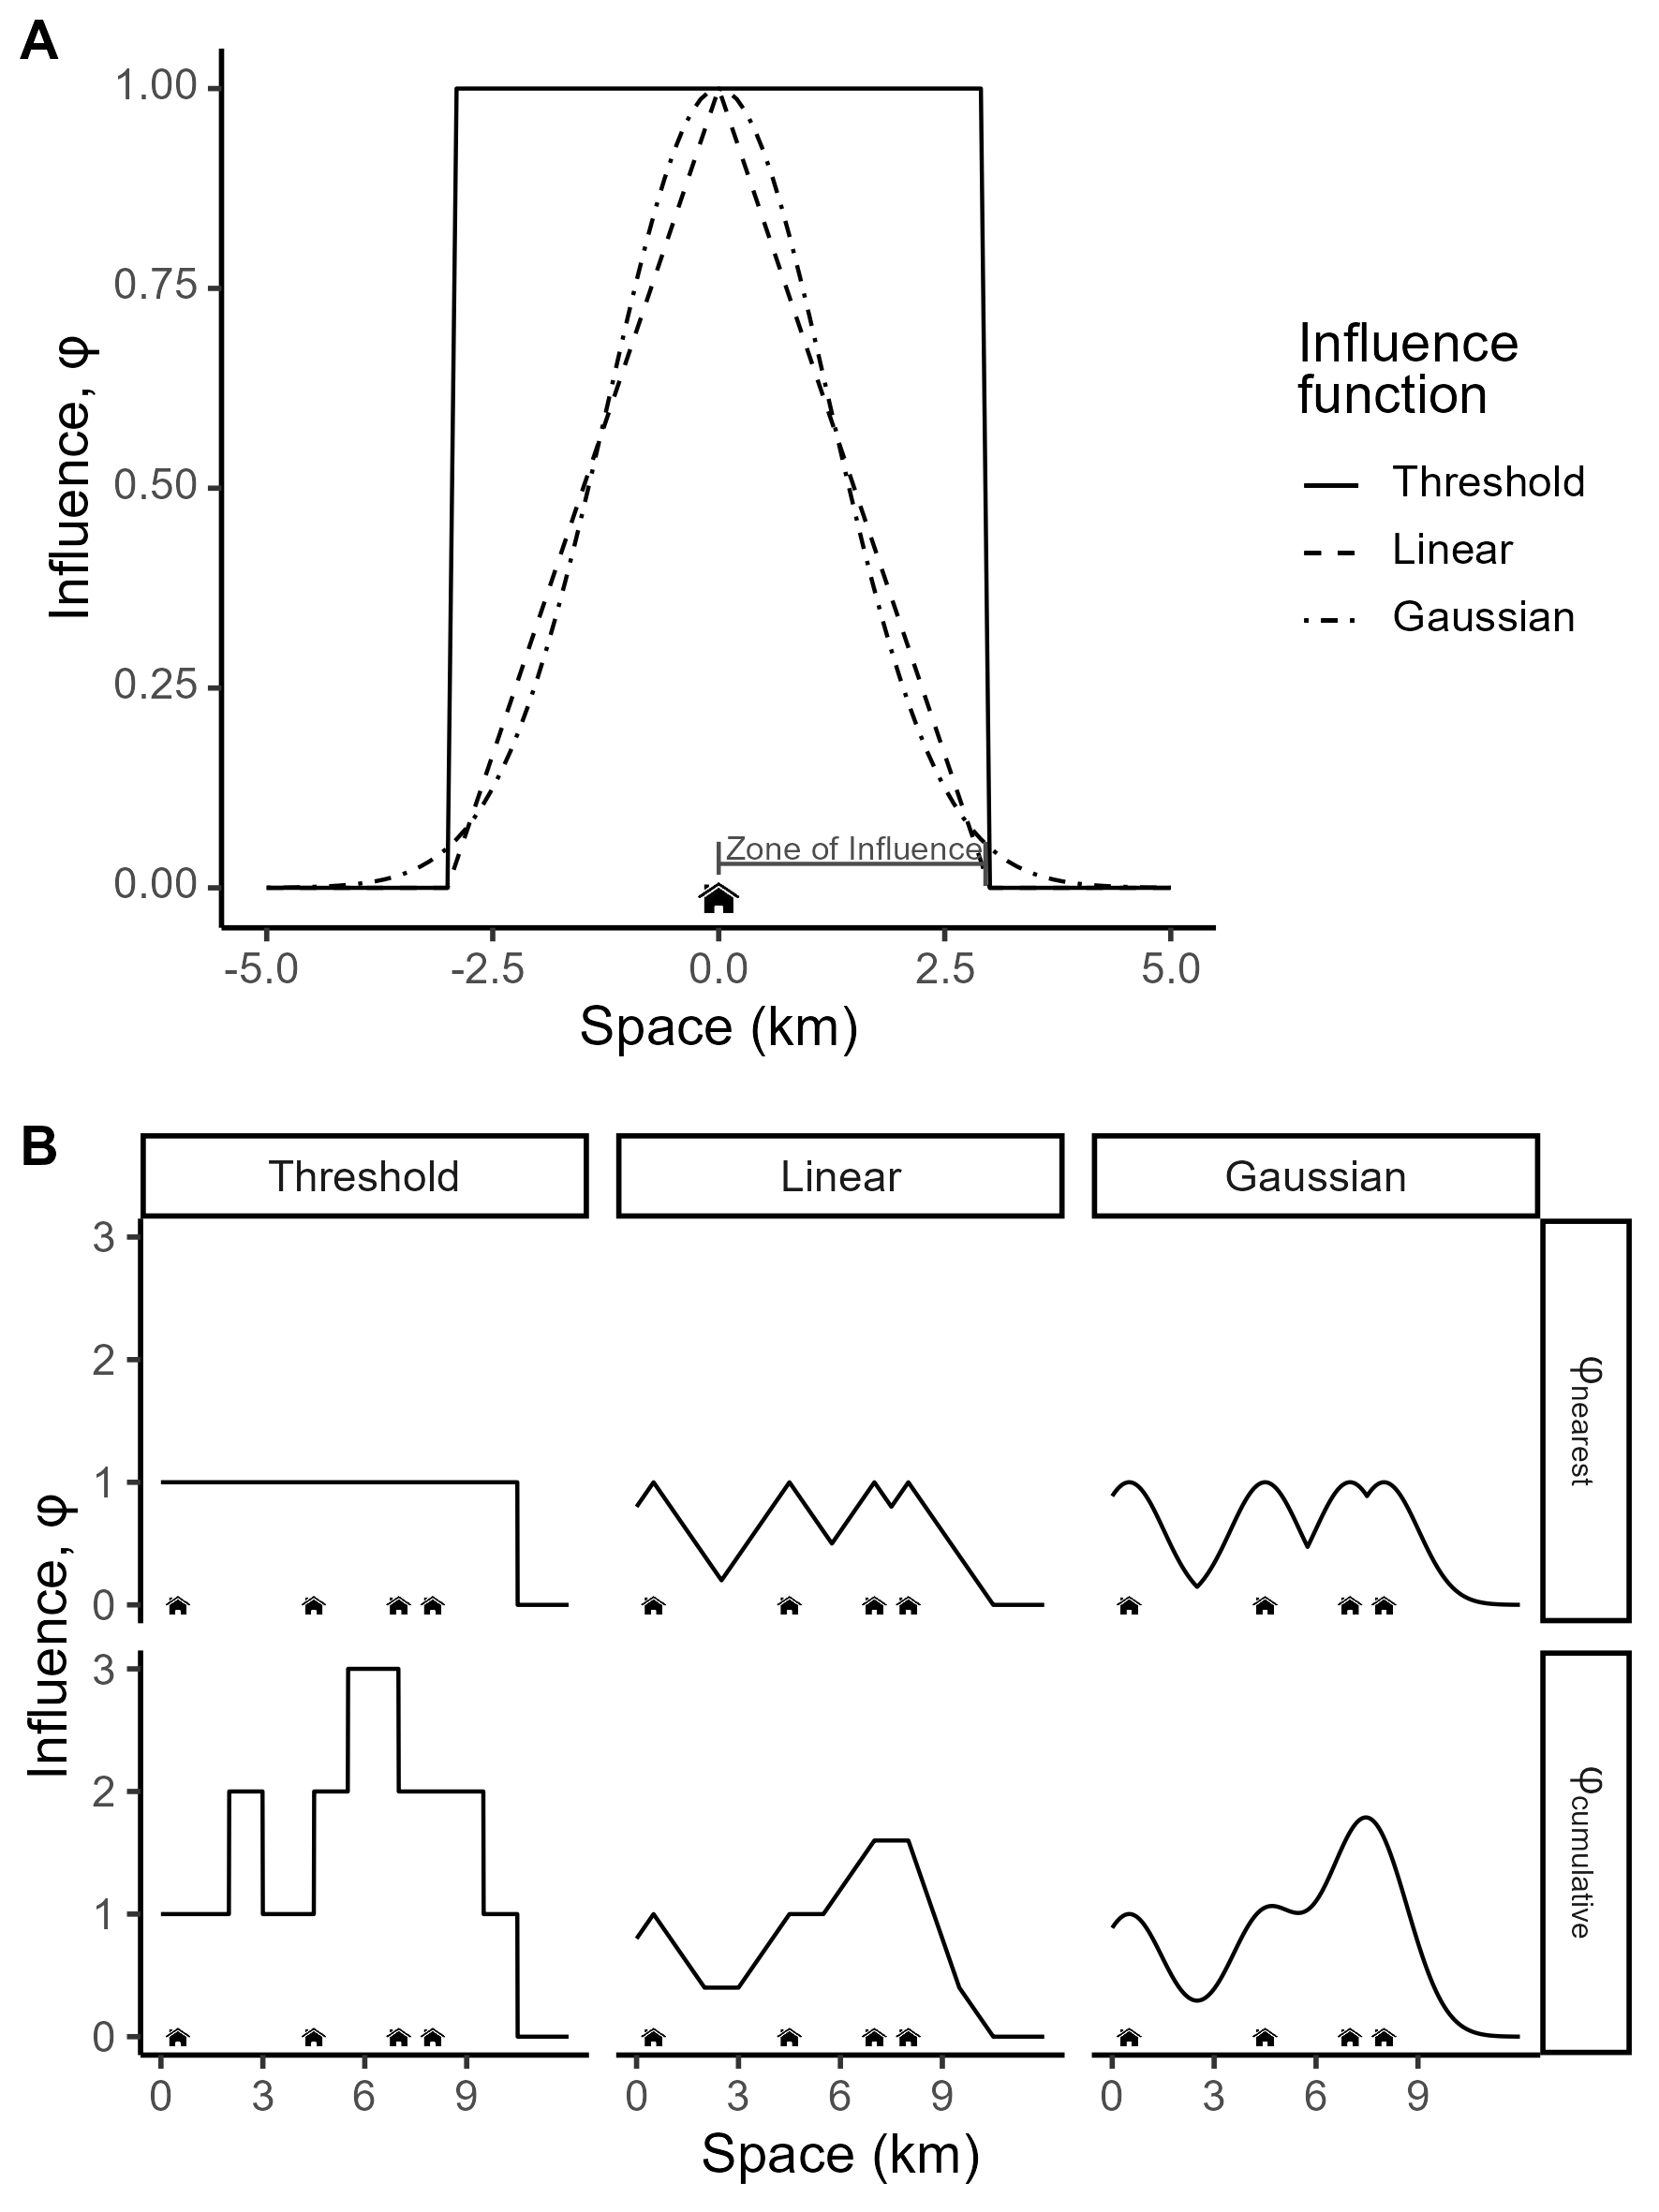
\includegraphics[width=0.9\textwidth]{figures/ZoI_conceptual.png}
\caption{\label{fig:zoi_conceptual} Illustration of the influence ($\phi$) of infrastructure features against the distance from those features ($d$), simplified for one dimension and using houses as an example. (A) Examples of influence functions according which the influence of the house might vary. A house has only an influence within its zone of influence (here $ZoI_{i_k} = 3 \text{ km}$). For the threshold function, the influence remains constant within the ZoI and drops to zero beyond it, whereas for both the linear and Gaussian functions it declines monotonically within the ZoI. 
%For functions that asymptotically approach zero, a cutoff must be selected to characterize the ZoI (here the ZoI is the distance where the influence decreases to $\phi_{i_k} < 0.05$). 
(B) Representation of the influence of multiple houses by considering only the nearest feature ($\phi_{nearest}$, upper row) or the cumulative influence of multiple features ($\phi_{cumulative}$, bottom row), for different influence functions. If only the nearest house is considered, the influence does not exceed one; when all houses act cumulatively, their cumulative influence can be much higher than one.}
\end{figure}

To translate those representations into a mathematical form, now we decompose each of the effect terms (i.e. A, B, C, ...), in equation \ref{eqn:HSF}. Suppose that in the landscape there are $n_k$ features of the same type of infrastructure $k$, and let the influence of the feature $i$ of an infrastructure \textit{k} follow an influence function \citep[or ``weighting function", ][]{miguet_how_2017} $\phi_{i_k} = f(d_{i_k}; ZoI_k)$, where $d_{i_k}$ is the distance to a feature ($i_k$) of infrastructure type $k$ and $ZoI_k$ is its zone of influence. Figure \ref{fig:zoi_conceptual}A shows a few possible shapes for the function $\phi_{i_k}$. We can sum the effect of each feature on animal habitat selection, so that the effects in equation \ref{eqn:HSF} become:

\begin{equation}
\label{eqn:HSFterm}
    E_k = \beta_k X_k = \sum_{i=1}^{n_k} \beta_{i_k} \phi_{i_k}
\end{equation}

Typically, only the nearest feature is considered, resulting on the implicit assumption that $\beta_i = 0$ for all $i > 1$ (where the features are ordered by increasing distance). Thus, eq. \ref{eqn:HSFterm} turns into:

\begin{equation}
\label{eqn:HSFnearest}
\begin{split}
    E_k & = \beta_{1_k} \phi_{1_k} \\
        & = \beta_{1_k} \phi_{nearest_k}
\end{split}                
\end{equation}

where $\phi_{nearest_k}$ is the influence of the nearest feature ($i = 1$) of the infrastructure type $k$ (see Fig. \ref{fig:zoi_conceptual}B). However, possibly a more reasonable assumption would be that $\beta_{i_k} = \beta_{{(i+1)}_k} = \beta_{{(i+2)}_k} = ... = \beta_k$, i.e. that all features of a given type present the same influence around them and all $\beta$'s are identical. Thus, eq. \ref{eqn:HSFterm} is reduced to:

\begin{equation}
\label{eqn:HSFcuminf}
\begin{split}
    E_k & = \beta_k \sum_{i=1}^{n_k} \phi_{i_k} \\
        & = \beta_k \phi_{cumulative_k}
\end{split}
\end{equation}

where $\phi_{cumulative_k} = \sum_{i=1}^{n_k} \phi_{i_k}$ is the cumulative influence measure and is proportional to 
%what has been called 
the ``density" of features in space \citep[e.g.][]{panzacchi_searching_2015}. The cumulative influence measure is easily calculated using geographical information systems, e.g. through neighborhood analysis, and can be rescaled to meaningful measurement scales, such as the number of point features per km\textsuperscript{2}. For the derivation of similar equations for variables represented as lines and areas, see Appendix A.

\section{Estimating the cumulative effects of multiple features}

In the cumulative effects assessment proposed here, the calculation of $\phi$ might be done before statistical analysis. In this formulation, $\phi$ defined based on different influence functions and ZoI are considered as different covariates (Fig. \ref{fig:workflow}). Therefore, the evaluation of how the effects of multiple infrastructure accumulate and the identification of the ZoI are recasted as a model selection rather than a parameterization problem.

\begin{figure}[h]
\centering
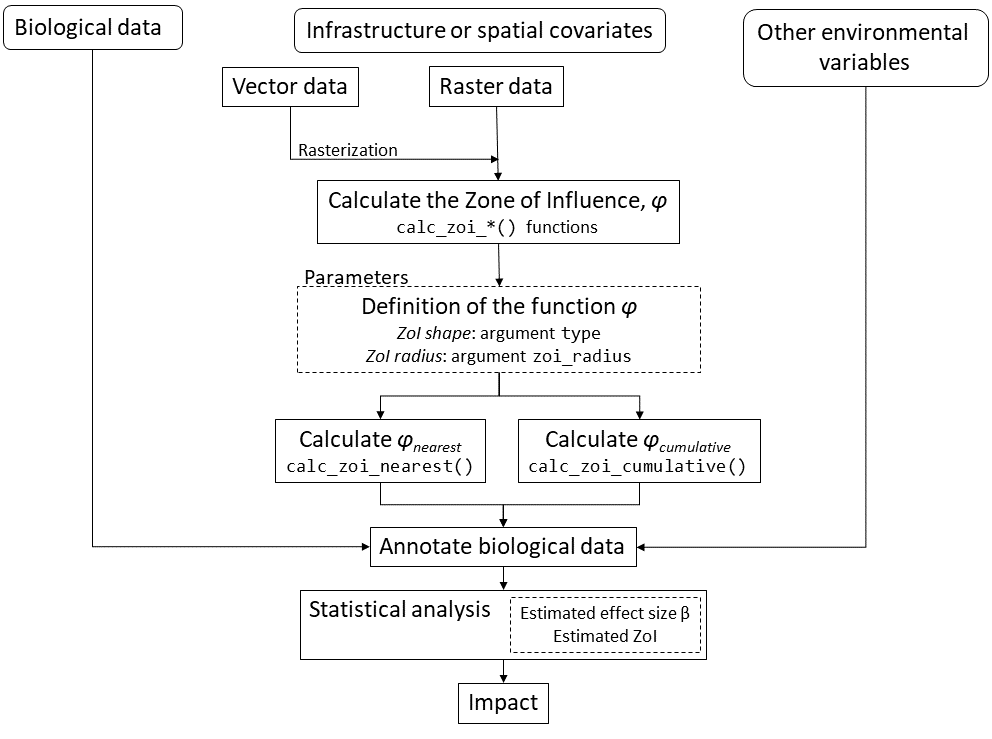
\includegraphics[width=1.3\textwidth,center]{figures/figure_workflow.png}
\caption{\label{fig:workflow} Workflow for calculating infrastructure influence $\phi$ and estimating the cumulative effects and ZoI of multiple infrastructure. Infrastructure raster data are input to the \texttt{calc\_influence} functions, which allow the calculation 
of $\phi_{nearest}$ and $\phi_{cumulative}$ based on arguments for the influence function shape and ZoI. The output influence rasters and other environmental data are then to annotate biological data and used in statistical fitting to estimate $\beta$ and ZoI for each infrastructure type.}
\end{figure}

To ease the use of the approach, we developed the \verb|oneimpact| R package. Based on raster maps with the location of infrastructure or other spatial variables, it allows the calculation of $\phi_{nearest}$ and $\phi_{cumulative}$ through the \verb|calc_influence_()| functions (Fig. \ref{fig:workflow}, Appendix D). The output influence raster maps are then used with other environmental data to annotate the biological data, and the estimation of the effect sizes $\beta$ and evaluation of the cumulative effects for different types of infrastructure is made through statistical fitting of eq. \ref{eqn:HSF} (Fig. \ref{fig:workflow}. To do so, one can use model selection, \citep{burnham_model_2002}, penalized regression \citep{lee_estimating_2020} or machine learning approaches, for example (REF?; Appendix D). Such statistical modeling procedures are beyond our scope, and we provide an example using model selection through AIC below (Appendix C).   

\section{When do the influence of the nearest feature $\phi_{nearest}$ and the cumulative influence $\phi_{cumulative}$ represent similar spatial variation?}

To interpret the two influence measures -- $\phi_{nearest}$ and $\phi_{cumulative}$ -- in ecological contexts, is it important to investigate in which conditions they are correlated and represent similar or different gradients of spatial variation. Similarities between the two variables depend on the spatial distribution of the infrastructure as well as their zone of influence, and might affect our ability to distinguish among their effects. To illustrate when they converge, we simulated $30 \times 30$ km\textsuperscript{2} landscapes with a constant number of point features (e.g. houses, cabins, turbines; $n = 100$) distributed following different spatial patterns, in a gradient of clustering, from regular and random to clustered (Fig. \ref{fig:simulated_landscapes}; Appendix B). For each landscape we calculated $\phi_{nearest}$ and $\phi_{cumulative}$ assuming a range of values for ZoI (from 0.06\% to 40\% of the landscape extent), using a linear decay function (Fig. \ref{fig:zoi_conceptual}). We then compared the resulting spatial patterns of $\phi_{nearest}$ and $\phi_{cumulative}$ through Pearson correlation of the values of the two measures at the same coordinates. 

\begin{figure}[h]
\centering
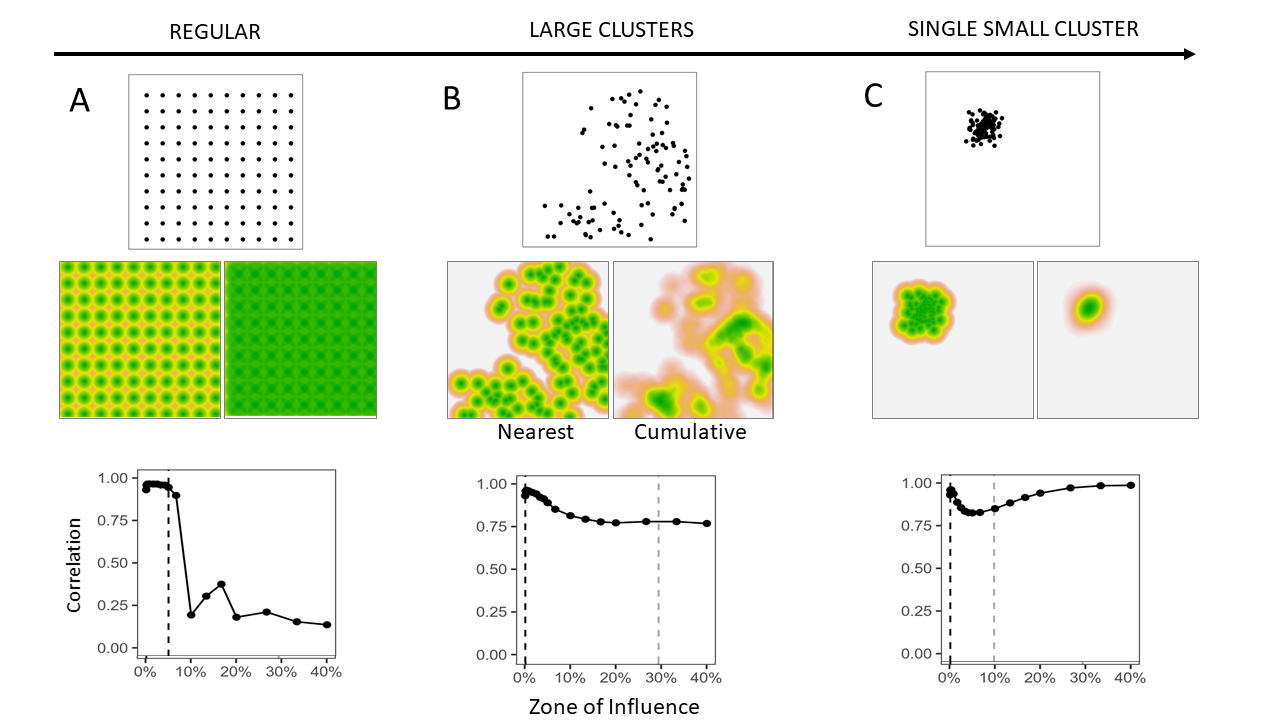
\includegraphics[width=1.3\textwidth,center]{figures/simulated_landscapes.png}
\caption{\label{fig:simulated_landscapes} Representation of the influence of nearest feature ($\phi_{nearest}$) and the cumulative influence ($\phi_{cumulative}$) in landscapes with point infrastructure spatially distributed in a gradient of clustering, from (A) a regular distribution 
%(e.g. a large solar power plant in a flat area) 
to (B) a set of clusters 
%(e.g. a wind industrial area formed by wind turbines built in the mountain tops) 
to (C) only one cluster. 
%(e.g. isolated village or urban center). 
The central panel shows a visual comparison between $\phi_{nearest}$ (left) and $\phi_{cumulative}$ (right) when $ZoI$ is 10\% of the landscape extent. The lower panel shows the correlation between $\phi_{nearest}$ and $\phi_{cumulative}$ in each landscape, as their ZoI increases. The dashed vertical lines show half the the minimum distance between features (black), beyond which there are cumulative effects of the different infrastructure, and the size of the feature clusters (grey), beyond which the correlation stops decreasing.}
\end{figure}

When $2 \times \text{ZoI}$ is smaller than the minimum distance between features, $\phi_{nearest}$ and $\phi_{cumulative}$ are identical (Fig. \ref{fig:simulated_landscapes}; $\text{correlation} = 1$ for all ZoI values below the black dashed vertical line). This happens when the ZoI of each feature is too small to overlap (Fig. 2A). When the ZoI increases, the effect of nearby features starts to accumulate and $\phi_{nearest}$ start to differ from $\phi_{cumulative}$. This is independent of the scenario for random, regular, and slightly clustered distributions of infrastructure features (Fig. \ref{fig:simulated_landscapes}A,B, Figs. B5 and B8). In contrast, as the features get more clumped and distributed in smaller clusters (up to a limit with a single small cluster, Fig. \ref{fig:simulated_landscapes}C), the correlation between $\phi_{nearest}$ and $\phi_{cumulative}$ goes through a point of inflection as the ZoI increases, beyond which it increases with ZoI (Fig. B5D-F). The point where the correlation stops decreasing is defined by the size of the clusters (grey dashed vertical line in Figs. \ref{fig:simulated_landscapes}B,C). For ZoI values larger than the cluster size, $\phi_{nearest}$ and $\phi_{cumulative}$ start to converge again. %This happens because the variation in cumulative influence increases continuously with ZoI and the variation in the influence of the nearest feature tends to get stable for large enough ZoI values (Figs. B5 and B7). 
This is when it might get hard to distinguish between the effect of each feature alone, regardless of the influence measure, and the effect of a collection of features transforms into that of a ``super-feature" (e.g. groups of houses or wind turbines behave as urban areas or wind parks, respectively). 
When the correlation between $\phi_{nearest}$ and $\phi_{cumulative}$ is higher, it might be difficult to distinguish if the impacts of a given infrastructure type accumulate or not. 
%However, in other cases (such as the correlation inflection point mentioned above) it might be easier to detect differences and test for cumulative effects.
However, whether a given biological response variable is affected by the nearest feature or by the cumulative influence of multiple features (or none) remain an empirical question to be explored in real landscapes. 

\section{Empirical demonstration on reindeer habitat selection}

\subsection{Study area, ecological data, and methods}

In our empirical demonstration we assessed the effects of multiple infrastructure on the Hardangervidda reindeer population in Norway using habitat selection during summer (Fig. \ref{fig:prediction_maps}). Reindeer are sensible to human activity, and the wild populations in Norway are the last remaining populations of this species in Europe. In summer, the area is visited by tourists and mountain hikers. There are 14,154 private cottages, 26 large tourist cabins, and hundreds of kilometers of trails in the area, besides roads and small tourist cabins (Fig. C2). We used GPS-tracking data from 48 (??) female reindeer collected in the month of July from 2001 to 2010 \citep[see][for further details]{panzacchi_searching_2015}. To assess reindeer habitat selection we used a use-availability setup, where each used GPS location was compared against nine available random locations spread within the area occupied by the population (Fig. \ref{fig:prediction_maps}). All locations were annotated with environmental covariates.

To account for bio-climatic-geographical variation in environmental characteristics we used the four first components from a principal component (PC) analysis conducted for whole Norway \citep{bakkestuen_step-less_2008}. They correspond to gradients of (1) PC1 - continentality, (2) PC2 - altitude, (3) PC3 - terrain ruggedness, and (4) PC4 - solar radiation. We included a quadratic term for PC1 and PC2 to account for niche ``optima" \citep[\textit{sensu}][]{panzacchi_searching_2015}. We also used a satellite-based land cover map with 25 vegetation classes, which were reclassified into 12 classes (see Table C2). To keep model fitting relatively simple and avoid correlation between covariates, we estimated the cumulative impacts for two anthropogenic variables: private cottages and large tourist cabins.

For the two infrastructure types we calculated both $\phi_{nearest}$ and $\phi_{cumulative}$ (Fig.~\ref{fig:zoi_conceptual}B) for ZoI ranging from 100 to 20,000 m. For each ZoI, we used four influence functions, to account for different shapes of the variation of the infrastructure influence within the ZoI (Fig.~\ref{fig:zoi_conceptual}A): threshold, linear decay, Gaussian decay, and exponential decay. To estimate reindeer habitat selection we fitted HSFs (eq. \ref{eqn:HSF}) using binomial generalized linear models \citep{fieberg_how_2021} with used and available locations as response and infrastructure, land cover, and bio-climatic variables as fixed effects. 

Model fitting consisted in two steps. We first fitted single-infrastructure models using variable selection procedure \citep{burnham_model_2002} to find the most likely influence functions $\phi$ and ZoI for each infrastructure type. Single-infrastructure HSF were fitted using the \verb|multifit| function in R \citep{huais_multifit_2018} and compared using AIC. Second, using the most likely influence functions $\phi$ and ZoI from the single-infrastructure models, we fitted multi-infrastructure HSF to assess the combined effects of multiple types of infrastructure, in an approach similar to \citet{laforge_process-focussed_2015}. 

To quantify the effects of infrastructure, we used eq. \ref{eqn:HSFterm} and multiplied the effect size -- the coefficients of the fitted model, $\beta$ -- by the influence measure $\phi$ included the model. We then estimated habitat suitability predicting the HSF (eq. \ref{eqn:HSF}) over the study area and rescaling the predicted values to the interval [0, 1]. For details on the data, environmental covariates, modeling, and results, see Appendix C.

\subsection{Cumulative effects on reindeer habitat selection}

Overall, both single- and multi-infrastructure models including $\phi_{cumulative}$ performed much better than models including $\phi_{nearest}$ (Table C2). This presents a strong evidence that the effects of private cottages and tourist cabins accumulate over reindeer habitat selection, making them avoid these infrastructures. As a comparison, the most plausible model including $\phi_{nearest}$ was ranked 26\textsuperscript{th} in the model selection ($\Delta AIC = 921$), and the most likely model including the log-distance to the nearest feature was ranked 44\textsuperscript{th} ($\Delta AIC = 1197$, Table C2).

The most parsimonious model showed private cottages exerted a constant cumulative influence within a ZoI of 10 km (threshold function) and large tourist cabins followed an exponentially decaying cumulative influence within a ZoI of 20 km (Fig. \ref{fig:impact_plot}; Table C2). Notice that, as parameterized here, for the tourist cabins an exponential decay with ZoI of 20 km means
that the influence of tourist cabins decrease to half of its maximum value
at ca. 5 km from the infrastructure (Fig. \ref{fig:impact_plot}, Appendix A). 

\begin{figure}[h]
\centering
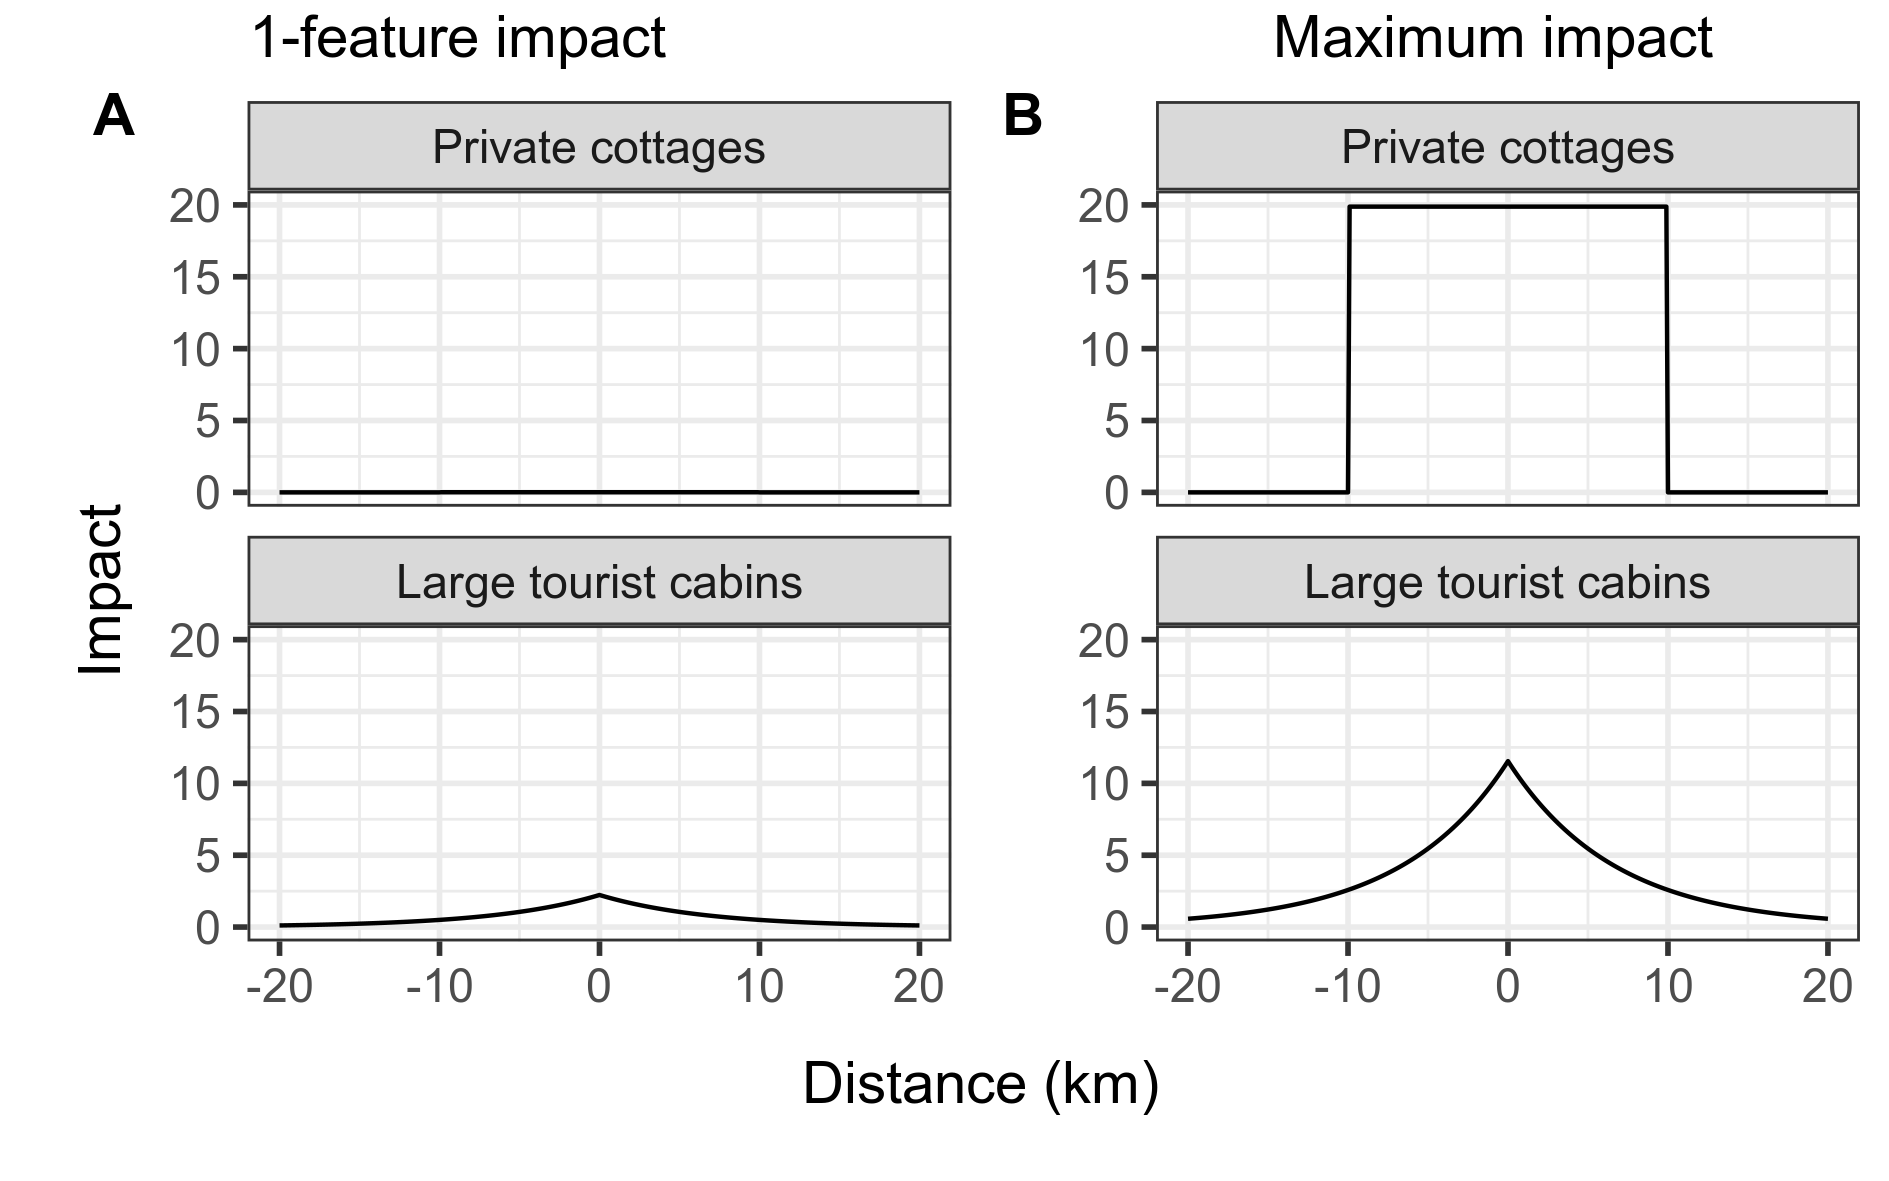
\includegraphics[width=1\textwidth,center]{figures/reindeer_zoi_impact_single_multiple_features.png}
\caption{\label{fig:impact_plot} Effect of private cottages and public cabins considering (A) only 1 feature and (B) the maximum number of features of each type of infrastructure in the study area (2664 for cottages, 5 for cabins). The effect is the product of the effect size (model coefficients, $\beta$) and the cumulative influence function ($\phi_{cumulative}$). While the effect of only one private cottage is negligible, at their maximum densities the cumulative effect of private cottages is higher than that of tourist cabins.}
\end{figure}

The estimated effect size of a single private
cottage ($\beta_{cottage} = -0.0081$) was much smaller than that of a single tourist cabin
($\beta_{\text{private cabin}} = -2.654$; Fig. \ref{fig:impact_plot}A, Table C3), as
private cottages were used by fewer people than the tourist cabins. However, as
private cottages occur at higher densities, in some areas their overall effect 
is larger than that of tourist cabins. In the areas where our most parsimonious model show the 
highest cumulative influence of infrastructure in Hardangervidda -- where the number of private cottages sum to 2664 
and the (exponentially weighted) number of tourist cabins sum to 5 -- the effect of 
private cottages clusters is nearly twice that of tourist cabins
 (Fig. \ref{fig:impact_plot}B and 4). Following the HSF coefficient interpretation from \citet{fieberg_how_2021}, considering that all other conditions are kept constant, a reindeer avoids an area 14.43 times more than an area with
330 fewer private cottages within a radius of 10 km. That is nearly the same difference in avoidance a reindeer presents among two areas 
that differ in 1 tourist cabin in a radius of 20 km (Appendix C).

When cumulative effects of infrastructure are predicted in space by multiplying the effect size and $\phi_{cumulative}$ (eq. \ref{eqn:HSFcuminf}), we see how the relative effect of private cottages and tourist cabins changes across space (Fig. \ref{fig:prediction_maps}). While the effect for private cottage rises to 20 in the areas with the highest cumulative influence of cottages, it hardly goes above 10 for tourist cabins. Because of the combined effect of multiple infrastructure, and given reindeer
avoided high densities of both infrastructure types at relatively large extents, 
areas of high habitat suitability for reindeer correspond to those in which the
cumulative influence of both infrastructure is low -- what matches the
locations used by reindeer, indicated through the GPS data (Fig. \ref{fig:prediction_maps}).

\begin{figure}[h]
\centering
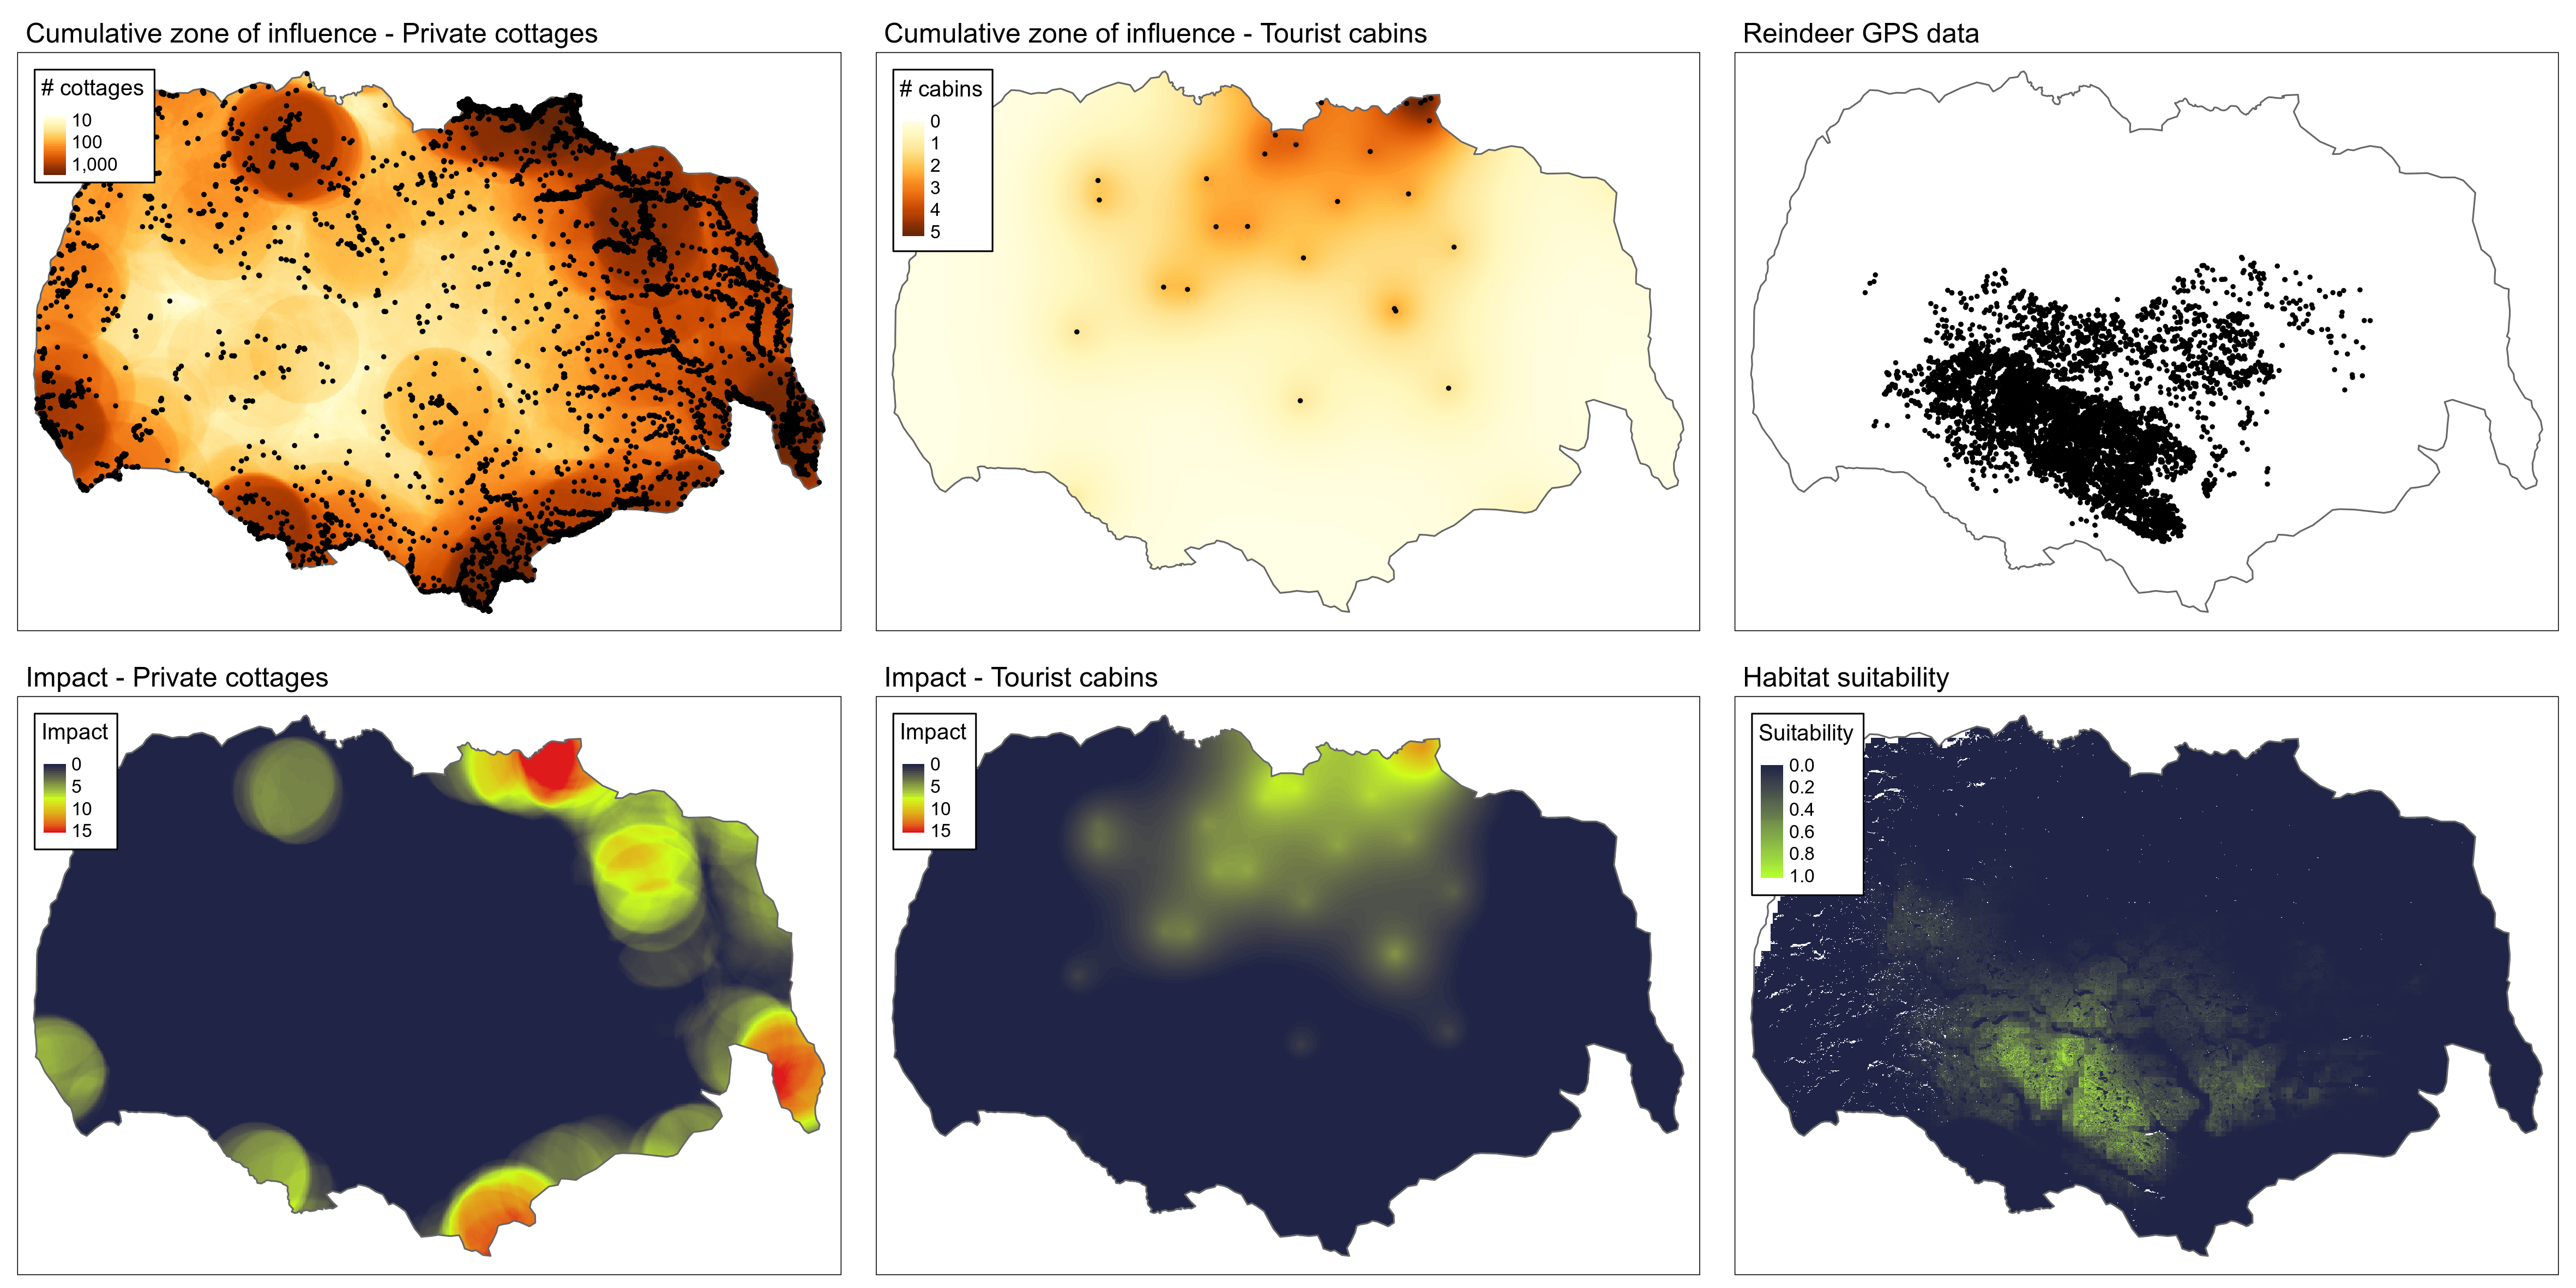
\includegraphics[width=1.3\textwidth,center]{figures/reindeer_results_prediction_maps.png}
\caption{\label{fig:prediction_maps} Maps of the most parsimonious cumulative influence variables $\phi_{cumulative}$ (private cottages: threshold with 10km ZoI; tourist cabins: exponential decay with 20 km ZoI) and their estimated effects on reindeer habitat selection. These maps are showed alongside the reindeer GPS locations in the Hardengervidda wild reindeer area and the estimated reindeer habitat suitability.}
\end{figure}

%\section{Tools to assess cumulative impacts of infrastructure}

%To ease the application of the cumulative effects assessment proposed here, we developed the \verb|oneimpact| R package. Based on raster maps with the location of infrastructure or any type of landscape variable (e.g. specific land cover or land use types), it allows the calculation of the influence from the nearest infrastructure feature ($\phi_{nearest}$ in eq. \ref{eqn:HSFnearest}) through the function \verb|calc_influence_nearest()| and the cumulative influence of multiple infrastructure ($\phi_{cum}$ in eq. \ref{eqn:HSFcuminf}) through the \verb|calc_influence_cumulative()| function. Both functions can be run using different filters or decay shapes (argument \verb|type|) -- exponential decay, linear (Bartlett or tent-shaped) decay, Gaussian (or half-normal) decay, threshold (or step) influence -- for multiple zones of influence (parameter \verb|zoi|), with the decay functions being parameterized on the ZoI. Besides those pre-defined decay functions, it also allows one to create user-defined filters (weight matrices) for cumulative effects estimation through the function \verb|create_filter()|.

%Furthermore, the \verb|oneimpact| package allows the calculation of the influence measures on both R \citep{r_core_team_r_2020} and GRASS GIS \citep{grass_development_team_geographic_2017}. On the one hand, the implementation in R allows high accessibility to users, since R is the most used statistical tool by ecologists \citep{lai_evaluating_2019}. On the other hand, the package provides a direct link from R to the powerful algorithms of GRASS GIS, so the influence measure calculation might be performed for very large and fine-scale spatio-temporal datasets. An introduction to the essential functions to calculate the two influence measures is found in Appendices D (for R) and E (for GRASS GIS). The \verb|oneimpact| package is available in the Github repository: \url{github.com/NINAnor/oneimpact}.

%\todo[inline]{Should we include a table with the functions and a short description?  Function name, description, type methods, input, output. Maybe in Appendix D.}

\section{Discussion}

There is an urge to evaluate, debate, and inform scientists, decision-makers, and the general public about the past, current, and future effects of global infrastructure on biodiversity \citep{laurance_conservation_2018}. Most of the decisions and regulations made for infrastructure projects are carried out with little knowledge about the potential, multiple impacts on the ecosystems where they are built and on the species living therein. Even when environmental impact assessments are well conducted, they hardly estimate the cumulative effects of new infrastructure with existing infrastructure or new infrastructure planned in parallel \citep{laurance_roads_2017, johnson_regulating_2011}. Current approaches and tools still lack in incorporating cumulative impacts \citep[but see][for recent advances]{gillingham_integration_2016}. Thus, building upon previous frameworks to understand cumulative effects \citep{naugle_unifying_2011} and adapting concepts and tools from landscape ecology literature to measure the influence of the nearest and of multiple features ($\phi_{nearest}$ and $\phi_{cumulative}$), here we present a way forward to clearly assess cumulative effects on biodiversity. 
%Here we depicted scenarios where each of the influence measures might converge or diverge, presented a case study to illustrate it, and offered tools to allow their application in ecological studies and environmental impact assessments.

\subsection{Applying the cumulative effects approach to impact assessment}

In our empirical demonstration using wild reindeer in Norway, we found strong support for the hypothesis of cumulative effects of private cottages and tourist resorts on reindeer habitat selection, leading to large ZoI -- up to 20 km. Quantifying effects based on effect sizes and influence functions $\phi$ allows us to compare as well as to combine the effects of different types of infrastructure. Our results show that the effect of a single cottage is smaller than that of a single tourist cabin, but that the effect of several aggregated private cottages may be much larger than that of tourist cabins (Fig. \ref{fig:impact_plot} and \ref{fig:prediction_maps}, Fig. C5). We also found less support for all models based only on the influence of the nearest feature ($\phi_{nearest}$) compared to the models incorporating the cumulative influence of multiple features ($\phi_{cumulative}$). This includes the models based on the log-distance to the nearest feature, which is a common proxy for the effect of infrastructure and landscape variables in the ecological literature \citep[e.g.][]{torres_assessing_2016,polfus_identifying_2011}. This means that, by limiting measures of infrastructure influence to the nearest feature only, researchers and practitioners have been ignoring the possibility of cumulative effects in ecological studies and impact assessments, what limits our overall understanding of the impacts of landscape change on biodiversity.

Three points must be highlighted regarding the interpretation of the ZoI.
First, if influence functions with different shapes are found to affect the ecological response under study, the ZoI represents distinct areas affected by infrastructure. For instance, while we found a constant influence (threshold function) of private cabins in a ZoI of 10 km, for tourist cabins we found the influence  decays exponentially with distance, which means the ZoI of 20 km around the resorts are not affected homogeneously. Therefore, understanding the effect of infrastructure across space requires us to combining the effect size and the influence function $\phi$ that represents the spatial component of the effect (eq. \ref{eqn:HSFterm}, Fig. \ref{fig:impact_plot} and \ref{fig:prediction_maps}). Second, since within the ZoI the influence might vary according to different shapes, the area affected by infrastructure of a given type might drastically change. Indeed, in a study with bird and insect abundance, \citet{miguet_how_2017} showed that the area affected by landscape variables can increase by a factor of up to 5.7 when using a distance-weighted influence measure (as the exponential and the Gaussian decay functions used here), in comparison to a threshold-based landscape measure. Third, given that the estimation of $\beta$ and $\phi$ is independent, the most likely ZoI can differ significantly between $\phi_{nearest}$ and $\phi_{cumulative}$, depending on the abundance and spatial distribution of features. For private cottages, which are present at high densities in our study area, the estimated ZoI for $\phi_{cumulative}$ was 10 km and the effect size was small (Fig. C3). In contrast, if only the nearest feature was considered ($\phi_{nearest}$), the estimated ZoI would be ten times lower (~1 km) and the effect size would be several orders of magnitude higher. This was not the case for tourist cabins, however, which are scarce and sparsely distributed in the study area (Fig. C4).

%For illustrative purposes, we used data from the wild reindeer population in Hardangervidda and included only two types of infrastructure. However, \citet{panzacchi_searching_2015} suggest that estimates of species niches and responses to infrastructure can be poor when based on single populations. For more comprehensive analyses, we suggest that habitat selection models, ecological niche models, occupancy or other ecological models using this approach to consider biological data from different populations and areas, to include as much as possible variation on landscapes and allow the estimation of cumulative functional responses in impact assessment of infrastructure over ecological processes.  

\subsection{Assumptions, advantages, and limitations of the approach}

As formulated here, the influence of the nearest feature ($\phi_{nearest}$, eq. \ref{eqn:HSFnearest}) and the cumulative influence ($\phi_{cumulative}$, eq. \ref{eqn:HSFcuminf}) are calculated before model fitting through the \verb|oneimpact| R package or through geographical information system tools (Fig. \ref{fig:workflow}). Here lies one of the main strengths of this approach: the cumulative effects of multiple features of an infrastructure are estimated through selection of models with either of the influence measures, for instance through model performance measures (e.g. AIC or $R^2$; \citealt{jackson_are_2015, huais_multifit_2018}), without the necessity of repeated model fitting and complex parameterization of non-linear functions \citep{lee_estimating_2020}. This allows one to estimate the influence function and the ZoI for several types of infrastructure. It also allows fitting models for large datasets \citep[millions of points, e.g.][]{tucker_moving_2018} encompassing large study areas and fine resolution landscape covariates, which makes the approach applicable over a wide range of fields in ecology. Furthermore, the pre-computation of $\phi_$ makes their visualization easy and their calculation computationally efficient and flexible.
%, allowing one to represent influence decays following different shapes \citep[e.g. threshold or exponential decay, as in ][]{miguet_how_2017}. 
% I could add something here about the discussion over model parameterization vs model selection for the definition of scales of effect, but I am not sure if it is worth it.

Our formulation of the influence functions $\phi$ follows two main assumptions. First, the ZoI is assumed to be constant regardless of the density of points in an area. A possibly more reasonable assumption would be to consider that the ZoI of a single or few features is smaller than that of a clusters of features, which are expected to be used by more people and cumulatively affect a wider area. Analogous calculations with variable function size have been implemented for decades in adaptive kernel density estimation [REF], so this premise can in principle be relaxed. Second, our formulation represents two extremes where only the nearest feature influences a focal ecological process ($\beta_i = 0$ for $i > 1$ in $\phi_{nearest}$) or all features affect the process equally ($\beta$ is constant over all features in $\phi_{cumulative}$). This is the simplest form of accounting for cumulative effects of multiple features of the same type. The advantage of this formulation lies on the independence between the magnitude of the impacts ($\beta$'s) and the influence functions ($\phi$), what makes it possible to pre-compute $\phi$ in GIS before model fitting. However, more complex formulations could be extended from eq. \ref{eqn:HSFterm}, for instance by considering that the influence of multiple features accumulate yet the closest one exerts a larger influence than features far away (higher $\beta$ for the nearest feature).

Through simulations, we showed that $\phi_{nearest}$ and $\phi_{cumulative}$ represent similar gradients of spatial variation when the spatial distribution of infrastructure features is sparse and the ZoI is small (so that the features are too spaced for their effects to accumulate) and when the features are clustered and ZoI is large (in which case the clusters of features act as ``super-features", e.g. urban areas instead of houses; Appendix B). In these two situations, due to their correlation, we might be limited in distinguishing whether the effects of multiple infrastructure on biodiversity accumulate. This might be assessed prior to statistical analysis through the computation of $\phi_{nearest}$ and $\phi_{cumulative}$ with multiple ZoI and a careful evaluation of their correlations. However, as the ``true" ZoI of an infrastructure type is hardly known in advance for any system, we recommend a general approach of computing and using the two influence measures, to evaluate if there is evidence of cumulative anthropogenic effects in the different ecological systems and processes.

It is important to remark that the extent of the study area and the zones of influence to be tested must be carefully selected, especially in cumulative impact assessment where the interplay between multiple factors may produce complex setups. First, the effects of infrastructure on ecological processes might differ depending of the extent of the study area \citep{vistnes_matter_2008}. \citet{skarin_human_2014} showed that, depending of the temporal and spatial range of the study, the same type of infrastructure might vary in their effect on ecological response variables, from no effect to positive or negative effects. As we show here, the spatial configuration of features and the ZoI might also affect our ability to detect if the effects of infrastructure accumulate. 
Second, depending on the ecological response variable, the range of ZoI tested must encompass values much higher than the range size or even the average dispersal distance of an species \citep{jackson_what_2012}. If the ZoI values are not properly defined, the ``true" ZoI at which the ecological process being measured is affected might not be selected, and the resulting estimated ZoI might be wrong and mislead management and conservation policies based on that scientific inference \citep[e.g.][]{jackson_are_2015}.

\section{Conclusions}

There is an increasing need to include cumulative effects on environmental impact assessments and ecological studies. However, even when they are present, bringing concepts and theoretical frameworks into concrete and objective analyses to estimate cumulative effects is often challenging and left to the responsibility of either the analysts or the regulators that review impact assessments \citep{johnson_regulating_2011}. Our approach offers resources for ecologists, environmental agencies, and stakeholders dealing with impact assessment to build concrete estimates of cumulative effects of multiple features of an infrastructure and their zone influence. 
Even though the examples given here focused on animal space use, the cumulative effect approach we presented is applicable over a wide range
of fields within ecology. Our formulation can be easily adapted to model other types of biological responses, such as population abundance \citep[e.g.][]{benitez-lopez_impacts_2010},
species richness \citep[e.g.][]{ficetola_ecological_2009} or other measures of biological diversity and ecological processes REF[e.g.], with direct application in environmental and strategic impact assessment and integrated land use planning.
      
\section*{Authors’ contributions}

BBN, BVM, and MP conceived the idea, designed the methods, and analyzed and discussed the data. BBN, BVM, MP, TT, KL, and OS provided data. BBN and BVM wrote the first draft. All authors contributed with discussions and to the final version of the manuscript.

\section*{Acknowledgements}

We thank P. Dodonov and M.H. Vancine for discussion around the implementation of the cumulative influence measures in R and E. Gurarie for the incentive and teachings on how to build an R package. We also thank NINA (or specific people) for the GPS data collection and management. The work presented here is the result of large projects supported by the Research Council of Norway (OneImpact, RenewableReindeer, ProdChange). BBN, AS, PS, and MA were also supported by a grant from the Swedish Energy Agency within the research programme Vindval (grant n. 46780-1) and by project MineDeer (Vinnova project n. 2019-05191).

\section*{Conflicts of Interest}

The authors declare no conflicts of interest.

\section*{Data availability statement}

GPS data is archived in Movebank (www.movebank.org) and might be accessed upon request. All environmental data was retrieved from public repositories. The \verb|oneimpact| package is open and available at \url{github.com/NINAnor/oneimpact}, and all scripts used in the analyses are available in the Github repository \url{github.com/bniebuhr/cumulative_influence_paper} (to be made public upon the acceptance of the manuscript).

\section*{Supplementary Material}

Appendix A. Deriving the cumulative influence for line and polygon representations of infrastructure. \\
Appendix B. Comparing the the influence of the nearest feature with the cumulative influence of multiple features \\
Appendix C. Cumulative effects of infrastructure on reindeer space use: fitting habitat selection models \\
Appendix D. Getting started with \verb|oneimpact|. \\
Appendix E. Calculating cumulative influence in GRASS GIS using the \verb|oneimpact| package in R.

\bibliographystyle{besjournals}
\bibliography{cuminf_bib}

\end{document}
